
%==================section 1 Introduction====
\section{Introduction}

   %\begin{figure}[h]
    %  \begin{floatrow}
    %  \ffigbox{\caption{SIR}\label{fig:sir}}{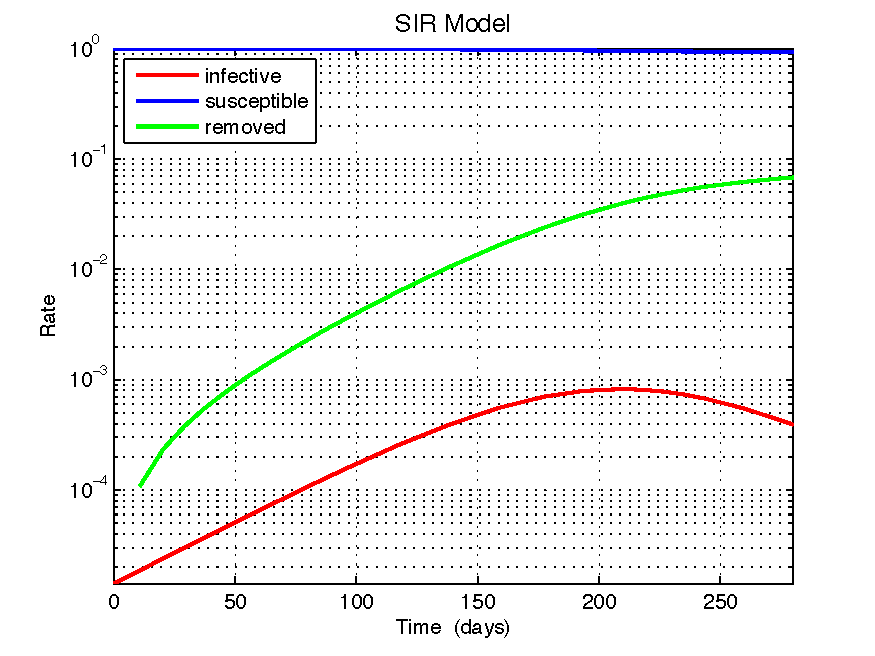
\includegraphics[width=1cm]{figure1.pdf}}
     % \ffigbox{\caption{SIQR}\label{fig:siqr}}{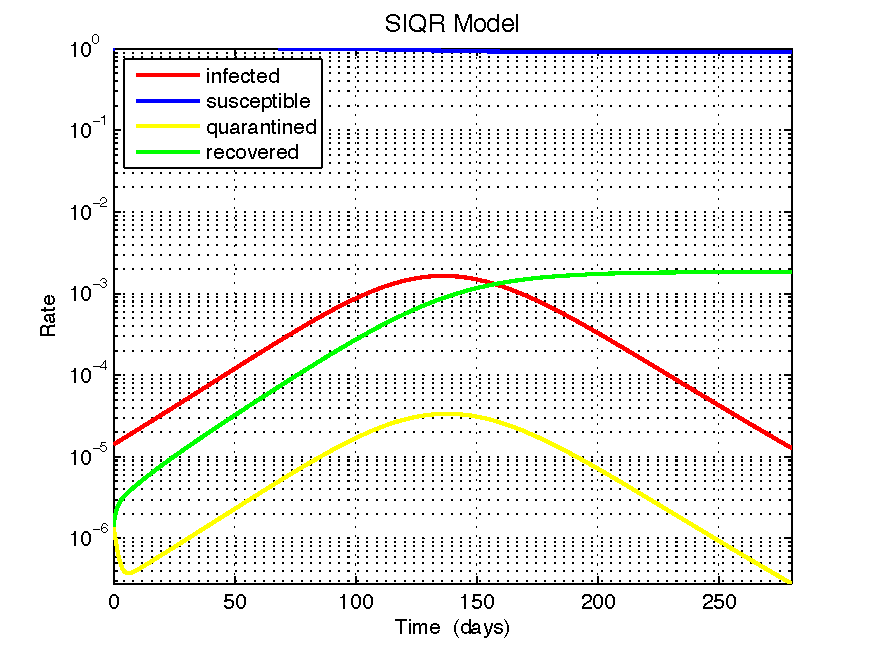
\includegraphics[width=1cm]{figure3.pdf}}
     % \end{floatrow}
    %\end{figure}

  \subsection{Background}
    Post-secondary education attainment has been playing a more and more important role in effecting not only the earning power of individuals but also the quality of their lifetime nowadays. An investigation shows that a worker with a bachelor's degree earns 84\% more than a worker without a degree - an average value of \$2.8 million over the course of a lifetime\cite{url1}.

	Among the various financial sources of schools, donations from individuals and foundations have been approved to be much helpful to improve education quality and student performance. Famous charitable foundation such as the Gates foundation and the Lumina foundation provide projects covering many aspects in post-secondary education, with policies varying from one state to another.

   However, with limited funding and limitless demanding, the investing plan should be as optimal as possible to get greatest returns on investment. In this way, the investment objects and the amount of economic support should be determined according to their capability of effectively using funding. And the time duration should be appropriate to get the strongest effect while the objects all get enough support. ROI also must be defined for foundations to make effect analyzing. Mathematical models can help in this procedure which would make sure every factor be well considered.


  \subsection{Planned approach}

	Since the information of candidate schools has been given including so many aspects such as costs, students' scores and graduates' financial situation, and the objects and amount should be determined. Analytic Hierarchy Process seems to conform to the demands, which can decompose a complex problem into a multilevel hierarchic structure of objectives, criteria, sub criteria and alternatives and provides a fundamental scale of relative magnitudes expressed in dominance units to represent judgments in the form of pairwise comparisons\cite{url2}.

In this model, the criteria contains the situation of school, performance of undergraduates and graduates. Factors given in database that can reflect these three aspects are picked up and set to be sub criteria. The AHP model then help ranking the schools to get more effect with limited investment.

To establish this complicated model, several points should be achieved.

\begin{enumerate}
	\item Given the related data of schools, return on investment is defined with several factors that can directly or indirectly show the effect of donation.
	\item These 12 factors are divided into three aspects and the relative weights and performance scores are evaluated and compared with each other.
	\item Through the AHP model, candidate schools are ranked by ROI expectation. Schools that will get donated and the amount of investment are determined with respect to reality. Then the initial invest plan comes out.
	\item ROI is estimated according to the initial plan and the ROI definition, the time duration of each donation is revised to get a better ROI.
	\item Sensitivity analysis is executed to get information about this model's response to data fluctuation. And the stability of this model is measured.
	\item Strengths and weaknesses of our model are identified. And we get more to do in the future after further discussion.
	\item By overviewing our approach, we get the conclusion of our work. Finally, we give a letter for the CFO of the Goodgrants Foundation.
\end{enumerate}


%=================subsection========
  \section{General assumptions}

	With the data of candidate schools in America, we make the following assumptions to complete the model. And these assumptions will also be applied our report.

	\begin{enumerate}
		\item The data of 2015 can represent the average situation of schools and students.
		\item Assume that the schools get donation will use all the investment into education and other aspects to improve students' performance.
		\item The differences of different states that may actually influent schools and students are not taken into consideration.
	\end{enumerate}

	The assumptions above are made to simplify the problem and fit it into the model.

%==================section 2 data clean
\section{Data cleaning}
	Data Cleaning is an essential part of data analysis and data mining. It plays an important role in Data science. For this problem, large amounts of data with imappropriate format make it hard to analysis and calculate in computer processing.

	Data cleansing differs from data validation in that validation almost invariably means data is rejected from the system at entry and is performed at entry time, rather than on batches of data\cite{url9}.

	Some data cleansing solutions will clean data by cross checking with a validated data set. Also data enhancement, where data is made more complete by adding related information, is a common data cleansing practice. For example, appending addresses with phone numbers related to that address\cite{url10}.

	What should be done first is to clean the whole data file. Data cleansing differs from data validation in that validation almost invariably means data is rejected from the system at entry and is performed at entry time, rather than on batches of data.


	\subsection{Single imputation with linear regression}

	The data file contains too much 'NULL' and 'PrivacySuppressed', it's essential to choose a suitble measure to correct this data file or the missing data may draw tolerance into the result of analysis.

In general, the missing data could be processed in many ways, such as Single imputation and Multiple imputation\cite{url8}. In this problem, linear regression of Single imputation could meet the demand well. So a linear regression model is built to predict the missing data in 3-year repayment rate, Median earnings of students and Share of students earning over \$25,000
\subsection{The procession of linear regression}
\begin{enumerate}
\item As there may be some nonlinear elements, the data sets need to be mapfeatured first.
In this step, the feature mapping function map the features into polynomial terms, returns a new feature array with more features, comprising of $X_1, X_2, {X_1}^2, {X_2}^2, X_1*X_2, {(X_1*X_2)}^2$, etc.
\item There are some features that contains more than 1000 missing data, which need to be done with FeatureNormalize. As features differ by order of magnitude, first performing feature scaling can make gradient descent converge much more quickly. And FeatureNormalize contains two steps:

\subitem 1. Subtract the mean value of each feature from the dataset.
\subitem 2. After subtracting the mean, additionally scale the feature values by their respective 'standard deviations'.

\item To combat the overfitting problem, the regularized linear regression model could be used. In this circumstance, the cost function and gradient is determined by the following formula:
\begin{equation}
J(\theta) = \frac{1}{2m}\sum_{i=1}^{m}{\left(\sum_{j=0}^{n}x_{ij}\theta_j-y_i\right)}^2+\frac{\lambda}{2m}\sum_{j=1}^n\theta^2_j
\end{equation}
\begin{equation}
\boldsymbol{grad} = \frac{1}{m}\sum^m_{i=1}\left(\sum_{j=0}^{n}x_{ij}\theta_j-y\right)\boldsymbol{x_i} + \frac{\lambda}{m}\boldsymbol{\theta}(\theta_0=0)
\end{equation}

\item Learning parameters using \boldsymbol{$fminunc$}(Matlab Function:Find minimum of unconstrained multivariable functionexpand all in page)
\end{enumerate}
The results of learning parameters could be expressed with learning curve. Combine the trained  with the value of cost function in training set and cross validation set, we could get the reliable complete data set.

\subsection{Assessment of rationality of the model}
It's clear to learned that whether the result of this model is convergent or not from the cost function in training set. Looking into the cost of cross validation set can help on choosing more proper parameter $\lambda$. This section will be discussed specificly in Result analysis section, which will not repeat here.

%==================Section 3 ROI=========
\section{Return on investment(ROI)}
	Return on investment (ROI) is the benefit to the investor resulting from an investment of some resource. A high ROI means the investment gains compare favorably to investment cost. As a performance measure, ROI is used to evaluate the efficiency of an investment or to compare the efficiency of a number of different investments\cite{url3}.

	In this problem, ROI refers more to the latter- the improvement of students' performance, not the economic feedback for foundations, which means we could not accurately measure the ROI by money. So ROI need to be redefined with elements in the data sets.

	Besides it is necessary to eliminate meaningless factors, which may mislead the results. Because too many details may reduce the consistency or even make the results unrealistic. Predominant factors therefore should be picked up from the information provided. And here are 13 factors need to be considered, and those elements can be divided into three aspects. And these three aspects composed of 12 elements together define the return on investment.

\begin{enumerate}
	\item Fundamental conditions of school
	\item Predominant degree awarded. Which can reflect the academic level in general.
	\item Control of institution. Public universities and privately established schools really have differences in cost, scale, financial sources and so on.
	\item Locale of institution. Location of school and the surroundings may have some connection with the scale of school and its education quality.
	\item Enrollment of undergraduate degree-seeking students. The number of undergraduate students have something to do with the amount of economic support.
	\item Average net price for Title IV institutions/public institutions. When considering the support for schools, the cost of students must be involved.
	\item Achievements of undergraduates.
	\item Percentage of undergraduates who receive a Pell Grant. The Pell Grant can reflect the performance of a student on a certain degree.

	\item Percent of all federal undergraduate students receiving a federal student loan. This element shows the economic pressure of students in general.
	\item Median debt of completers, suppressed for n=30. Debt of completers may reflect the time that has been spent on school life. Students that concentrate on school life tend to have more debts than those meanwhile working outside.
	\item Median debt of completers expressed in 10-year monthly payments, suppressed for n=30.
	\item Achievements of graduates
	\item 3-year repayment rate, suppressed for n=30. The repayment can directly express the performance of graduates.
	\item Median earnings of students working and not enrolled 10 years after entry. Earnings can represent the return in general.
	\item Share of students earning over \$25,000/year (threshold earnings) 6 years after entry. This factor cooperate with the other two above to reflect the economic situation of graduates.

\end{enumerate}

One effective way to calculate the ROI overover these selected features is weighted sum approach. After pickingup 12 features, we will use the algorithm of the AHP to analyse data. Concretely, we will generate the weight vector using AHP Mode.

%==================section 2
\section{AHP model}
\subsection{Tradational AHP Model}
	the traditional analytic hierarchy process(AHP), which was originally developed by $Saaty$ in 1970s\cite{url4}, is a structured technique for organizing and analyzing complex decisions, based on psychology. It is a decision-making procedure widely used in management science, business, healthcare shipbuilding\cite{url5} and operations research for establishing priorities within the context of multi-criteria decision making. It help the decision makers to solve the problem by decomposing a complex problem into a multilevel hierarchic structure of objects, criteria, sub-criteria and alternatives and provides a fundamental scale of relative magnitudes expressed in dominance units to represent judgements in the form of pairwise comparisons\cite{url2}.

	After deriving a ratio scale of relative magnitudes that are expressed in priority units from each set of comparisons, an overall ratio scale of priorities is synthesized to rank the alternatives\cite{url6}. Three principles can be used to summarize the procedure of an AHP, which are decomposition, comparative judgements, and synthesis of priorities\cite{url7}.

	The AHP help decision makers find one that best suits their goal and their understanding of the problem.

	First, we decompose our decision problem into a hierarchy of more easily comprehended sub problems, every one of which can be analyzed independently. The elements of the hierarchy can relate to any aspect of the decision problem-tangible or intangible, carefully measured or roughly estimated, well or poorly understood- anything at all that applies to the decision at hand.

	Once our hierarchy is built, we systematically evaluate its various elements by comparing them to each two at a time, with respect to their impact above them in the hierarchy. In making the comparisons, we can use concrete data about the elements, but the typically use our judgments about the elements' relative meaning and importance. It is the essence of the AHP that human judgments, and not just the underlying information, can be used in performing the evaluations.

	The AHP converts these evaluations to numerical values that can be processed and compared over the entire range of the problem\cite{url13}. A numerical weight or priority is derived for each element of the hierarchy, allowing diverse and often incommensurable elements to be compared to one another in a rational and consistent way\cite{url2}. This capability distinguishes the AHP from other decision making techniques\cite{url13}.

	As can be seen in the material that follows, using the AHP involves the mathematical synthesis of numerous judgments about the decision problem at hand. It is not uncommon for these judgments about the decision problem at hand\cite{url4}. It is not uncommon for these judgments to number in the dozens or even the hundreds. While the math can be dozen by hand or with a calculator, it is far more common to use one of several computerized methods for entering and synthesizing the judgments\cite{url13}. The simplest of these involve standard spreadsheet software, while the most complex use custom software, often augmented by special devices for acquiring the judgments of decision makers gathered in a meeting room\cite{url13}.

\subsection{The typical procedure for using the AHP}

\begin{enumerate}
\item Model the problem as a hierarchy containing the decision goal, the alternatives for reaching it, and the criteria for evaluating the alternatives.
\item Establish priorities among the elements of the hierarchy by making a series of judgments based on pairwise comparisons of the elements.
\item Synthesize these judgments to yield a set of overall priorities for the hierarchy. This would combine the investors' judgments about location, price and timing for properties A, B, C and D into overall priorities for each property.
\item Check the consistency of the judgments.
\item Come to a final decision based on the results of this process.
\end{enumerate}

\subsection{Assessment of rationality of the model}
Consistence checking is a proven way to assess the AHP model. This section will be discussed specificly in Result analysis section, which will not repeat here.

\subsection{Data processing and results}

As has been explained before,12 elements have been picked up to reflect ROI. Now set the elements-Predominant degree awarded, Control of institution, Locale of institution, Enrollment of undergraduate degree-seeking students, Average net price for Title IV institutions、Percentage of undergraduates who receive a Pell Grant, Percent of all federal undergraduate students receiving a federal student loan, Median debt of completers, Median debt of completers expressed in 10-year monthly payments, 3-year repayment rate, Median earnings of students working and not enrolled 10 years after entry, Share of students earning over \$25,000/year (threshold earnings) 6 years after entry as sub-criteria C1-C12. And the 12 elements could be divided into three aspects: School(C1-C5), Undergraduates(C6-C9), graduates(C10-C12), which could be set as criteria B1-B3 \autoref{fig:ahp}.

    \begin{figure}[h]
      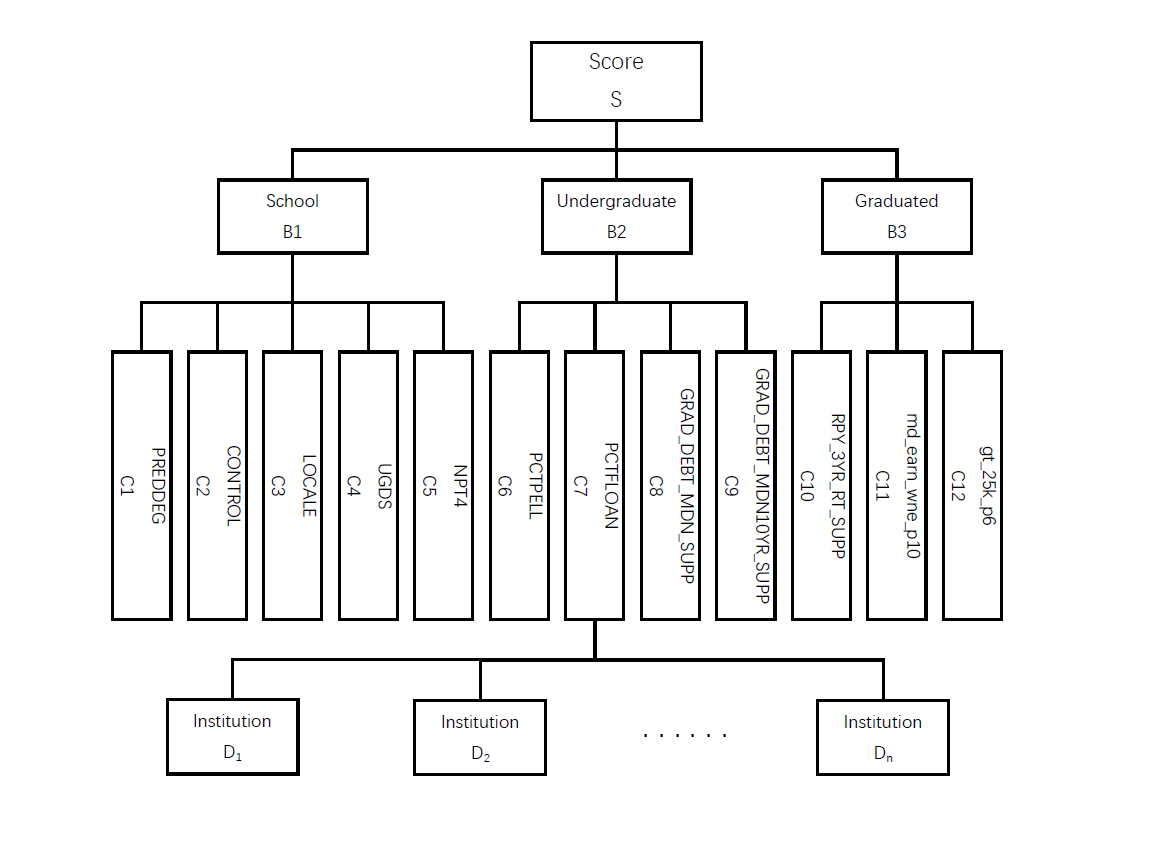
\includegraphics[width=15cm]{2016figure6.png}
      \caption{AHP model}\label{fig:ahp}
    \end{figure}
Through expert group judgement with rank policies from other professional ranking institutions, we get reciprocal matrix (judgement matrix) $mat_1$, $mat_2$, $mat_3$. Then through AHP, here comes out the eigenvectors (normalized) corresponding to max eigenvalues:

\begin{equation}
	\boldsymbol{w_1^{'}} = \begin{bmatrix}
0.4393 & 0.1045 & 0.0444 & 0.2245 & 0.1873
\end{bmatrix}
\end{equation}
\begin{equation}
	\boldsymbol{w_2^{'}} = \begin{bmatrix}
0.4444 & 0.1111 & 0.2222 & 0.2222
\end{bmatrix}
\end{equation}
\begin{equation}
	\boldsymbol{w_3^{'}} = \begin{bmatrix}
0.5396 & 0.1634 & 0.2970
\end{bmatrix}
\end{equation}

Then merge C1-C5 into $C_1$, C6-C9 into $C_2$, C10-C12 into $C_3$, we get:
\begin{equation}
\begin{bmatrix}
B_i
\end{bmatrix} = \begin{bmatrix} C_i \end{bmatrix} \times \begin{bmatrix} w_i\end{bmatrix} \,i=1,2,3
\end{equation}

Similarly, through expert group judgement, we get reciprocal matrix mat from $C_1$, $C_2$, $C_3$, and then we get the eigenvectors w' (normalized) corresponding to max eigenvalues through AHP agiain:
\begin{equation}
	\boldsymbol{w^{'}} = \begin{bmatrix}
0.6000 & 0.3000 & 0.1000
\end{bmatrix}
\end{equation}
% Table generated by Excel2LaTeX from sheet 'Sheet2'
\begin{table}[htbp]
  \centering
  \caption{The weight of items}
    \begin{tabular}{lr}
    \toprule
    \textbf{Item} & Weight \\
    \midrule
    \textbf{PREDDEG} & 0.26355 \\
    \textbf{CONTROL} & 0.062706 \\
    \textbf{LOCALE} & 0.02667 \\
    \textbf{UGDS} & 0.134692 \\
    \textbf{NPT4} & 0.112382 \\
    \textbf{PCTPELL} & 0.133333 \\
    \textbf{PCTFLOAN} & 0.033333 \\
    \textbf{GRAD\_DEBT\_MDN\_SUPP} & 0.066667 \\
    \textbf{GRAD\_DEBT\_MDN10YR\_SUPP} & 0.066667 \\
    \textbf{RPY\_3YR\_RT\_SUPP} & 0.053961 \\
    \textbf{md\_earn\_wne\_p10} & 0.016342 \\
    \textbf{gt\_25k\_p6} & 0.029696 \\
    \bottomrule
    \end{tabular}%
  \label{tab:item}%
\end{table}%

  \begin{figure}[h]
      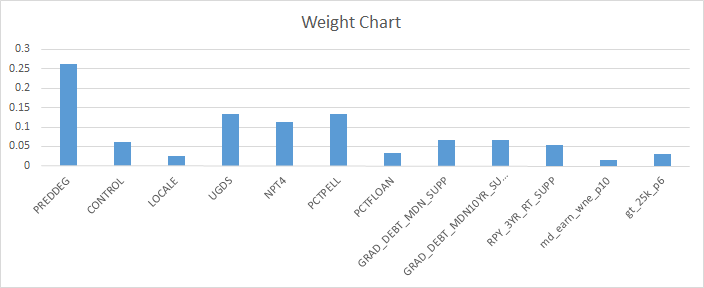
\includegraphics[width=15cm]{2016figure7.png}
      \caption{The weight chart}\label{fig:weight}
    \end{figure}
The score of top N schools and the amount of donation are shown in next chapter \autoref{tab:rank}:




%==========Section: Investment Strategy======
\section{Investment strategy}
	\subsection{Determining the value of N}
	As we've get the candidate school ranked by ROI scores, the priority and the corresponding weight of each school to get funding has been determined. But the amount of donation for each school still depends on how much schools will get invested. An appropriate method should be found to get more schools benefitted while every benefitted school get enough support.

	Assume that top N schools in the rank table will get investment, obviously the $1^{st}$ school get the most money and the Nst school get the least money. By analyzing the donation records of several schools, we get an conclusion that the least amount of money that will give a college enough help is about \$2,000,000, and \$5,000,000 million is the top limit of efficient investment. And we get the relationship between the most/least money and the number N chosen, which could be shown as following figures:

\begin{figure}[h]
      \begin{floatrow}
      \ffigbox{\caption{Most money recieved}\label{fig:most}}{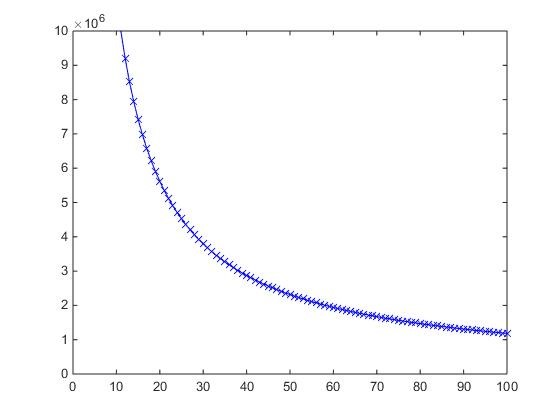
\includegraphics[width=8cm]{2016figure1.jpg}}
      \ffigbox{\caption{Least money recieved}\label{fig:least}}{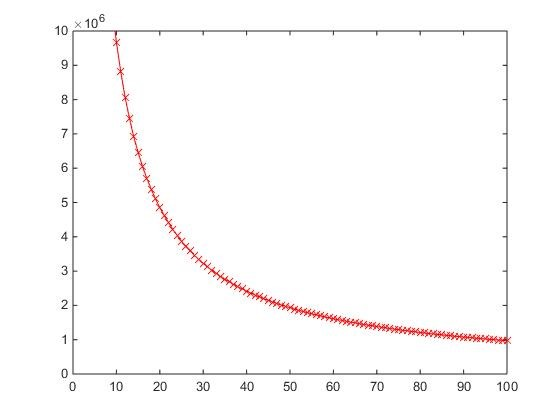
\includegraphics[width=8cm]{2016figure2.jpg}}
      \end{floatrow}
    \end{figure}

From these figures, we can see that the most/least money will decrease if N gets larger. According to the result above, the most money should not be more than \$5,000,000, and the least money should not be less than \$2,000,000. Combine with the figure, we can get the conclusion that 22 schools be invested should be the most effective and efficient way. With N = 22, the amount of money for every school is also determined.

	\subsection{Schools ranked by investment amount}
As the data sets will change as time goes by, the rank result will also get updated. The first year's invest plan is shown below \autoref{tab:rank}:

% Table generated by Excel2LaTeX from sheet 'Sheet1'
\begin{table}[htbp]
  \centering
  \caption{Schools ranked by investment amount}
    \begin{tabular}{cllr}
    \toprule
    \textbf{UNITID} & \multicolumn{1}{c}{\textbf{INSTNM}} & \multicolumn{1}{c}{\textbf{Score}} & \multicolumn{1}{c}{\textbf{Money}} \\
    \midrule
    232557 & Liberty University & 4.055349646 & 5120877.083 \\
    150987 & Ivy Tech Community College & 3.819812778 & 4823453.813 \\
    132903 & University of Central Florida & 3.735811479 & 4717381.498 \\
    214777 & Pennsylvania State University-Main Campus & 3.700081951 & 4672264.175 \\
    164872 & Boston Architectural College & 3.636278663 & 4591696.819 \\
    109651 & Art Center College of Design & 3.605513625 & 4552848.387 \\
    193900 & New York University & 3.603229283 & 4549963.843 \\
    133979 & Florida Memorial University & 3.596437466 & 4541387.502 \\
    133951 & Florida International University & 3.579236866 & 4519667.511 \\
    123952 & Southern California Institute of Architecture & 3.5691246 & 4506898.286 \\
    385619 & Everglades University & 3.566176079 & 4503175.053 \\
    204796 & Ohio State University-Main Campus & 3.552167052 & 4485485.208 \\
    171100 & Michigan State University & 3.549879846 & 4482597.047 \\
    102377 & Tuskegee University & 3.530919899 & 4458655.448 \\
    228778 & The University of Texas at Austin & 3.530853676 & 4458571.826 \\
    212054 & Drexel University & 3.521109863 & 4446267.862 \\
    186380 & Rutgers University-New Brunswick & 3.51945571 & 4444179.088 \\
    433387 & Western Governors University & 3.514403689 & 4437799.667 \\
    164988 & Boston University & 3.505537472 & 4426603.886 \\
    183026 & Southern New Hampshire University & 3.502775741 & 4423116.521 \\
    166656 & MCPHS University & 3.500158862 & 4419812.067 \\
    138947 & Clark Atlanta University & 3.498167442 & 4417297.41 \\
    \bottomrule
    \end{tabular}%
  \label{tab:rank}%
\end{table}%


%==================Section:===


%===========Analysis of the results============
\section{Analysis of the results}
\subsection{Stability analysis}
\paragraph{Stability analysis of linear regression}

In order to analyze the stability, we plot a learning curve and cross validation curve of error v.s. m and $\lambda$ as below\autoref{fig:learningcurve}:

 \begin{figure}[h]
      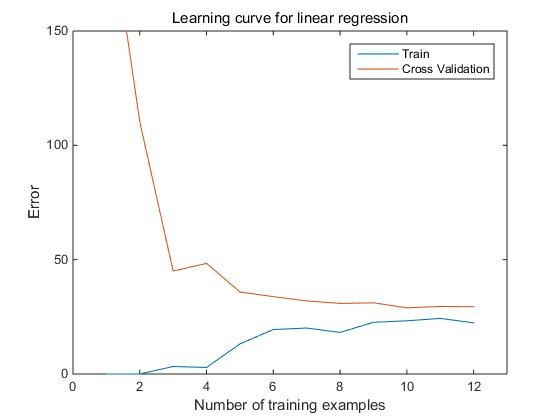
\includegraphics[width=10cm]{2016figure3.jpg}
      \caption{Learning curve for linear regression}\label{fig:learningcurve}
 \end{figure}

Learning curves is useful in debugging learning algorithms. It is observed that both the train error and cross validation error are high when the number of training examples is increased. This reflects a high bias problem in the model - the linear regression model istoo simple and is unable to fit our dataset well. In the next picture, after the implement of polynomial regression to fit a better model for this dataset, there will not be a gap between the training and cross validation errors, indicating a high variance problem.

the value of $\lambda$ can significantly affect the results of regularized polynomial regression on the training and cross validation set. In particular, a model without regularization ($\lambda = 0$) fits the training set well, but does not generalize. Conversely, a model with too much regularization ($\lambda = 100$) does not fit the training set and testing set well. A good choice of $\lambda$ can provide a good fit to the data.
 \begin{figure}[h]
      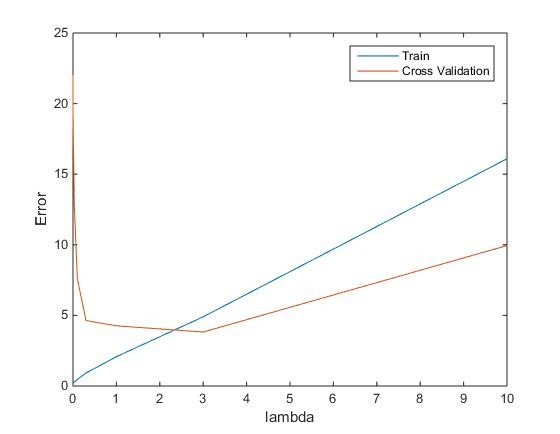
\includegraphics[width=10cm]{2016figure4.jpg}
      \caption{The cross validation curve}\label{fig:lambda}
 \end{figure}

Plotting the cross validation curve implement an automated method to select the $\lambda$ parameter (\autoref{fig:lambda}). Concretely, when using a cross validation set to evaluate how good each $\lambda$ value is, a proper $\lambda$ could be chosen. After selecting the best $\lambda$ value using the cross validation set, we can then evaluate the model on the test set to estimate how well the model will perform on actual unseen data.

In this figure (\autoref{fig:lambda}), we can see that the best value of $\lambda$ is around 3. Due to randomness in the training and validation splits of the dataset, the cross validation error can sometimes be lower than the training error.



\paragraph{Stability analysis of AHP}

In general, the reciprocal matrix is not consistent. But in order to use the eigenvectors corresponding to max eigenvalues as the weight vector of compared elements, the inconsistency should be in the allowable range.

But the larger that $\lambda$ is than n, the more severe that the inconsistency of matrix \boldsymbol{$A$} will be, and the error will be larger when regarding the eigenvectors as weight vectors. So the consistency index was defined by $Saaty$ as:

\begin{equation}
\boldsymbol{CI} = \frac{(\lambda - n)} { (n - 1)}
\end{equation}

As the standard of \boldsymbol{$CI$}, Saaty then came up with the concept of random index, \boldsymbol{$RI$} for short. \boldsymbol{$RI$} comes from the average of \boldsymbol{$RI$} of the reciprocal matrixes constructed randomly. The empirical value of RI is given in the table below (\autoref{tab:ri}):

% Table generated by Excel2LaTeX from sheet 'Sheet2'
\begin{table}[htbp]
  \centering
  \caption{The empirical value of RI}
    \begin{tabular}{rrrrrrrrrrrr}
    \toprule
    n     & 1     & 2     & 3     & 4     & 5     & 6     & 7     & 8     & 9     & 10    & 11 \\
    \midrule
    RI    & 0     & 0     & 0.58  & 0.9   & 1.12  & 1.24  & 1.32  & 1.41  & 1.45  & 1.49  & 1.51 \\
    \bottomrule
    \end{tabular}%
  \label{tab:ri}%
\end{table}%

Define \boldsymbol{$CR$} as the ratio of \boldsymbol{$CI$} and \boldsymbol{$RI$}, when
\begin{equation}
\boldsymbol{CR} = \frac{\boldsymbol{CI} }{\boldsymbol{RI}} < 0.1
\end{equation}

We can say that the inconsistency is in the allowable range, which means that it is reasonable to regard the eigenvectors as weight vectors.

% Table generated by Excel2LaTeX from sheet 'Sheet2'
\begin{table}[htbp]
  \centering
  \caption{The CR of 4 matrix}
    \begin{tabular}{rrrrr}
    \toprule
    CR    & $mat_1$ & $mat_2$ & $mat_3$ & $mat_4$ \\
    \midrule
    Value & 0.0445 & -0.0000     & 0.0079 & -0.0000 \\
    \bottomrule
    \end{tabular}%
  \label{tab:cr}%
\end{table}%


\begin{figure}[h]
      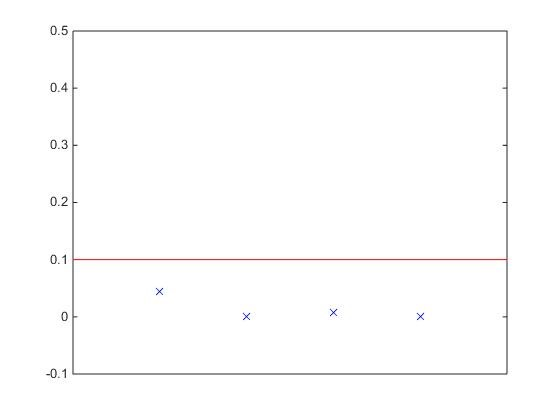
\includegraphics[width=10cm]{2016figure5.jpg}
      \caption{The CR of 4 matrix}\label{fig:cr}
 \end{figure}

According to the theory above, we can conclude that the inconsistency is in the allowable range, and it's reasonable to regard the eigenvectors as weight vectors.

%
%\begin{figure}[h]
%      \begin{floatrow}
%      \ffigbox{\caption{Sensitivity for $I(t)$ with $\beta$}\label{fig:figure11}}{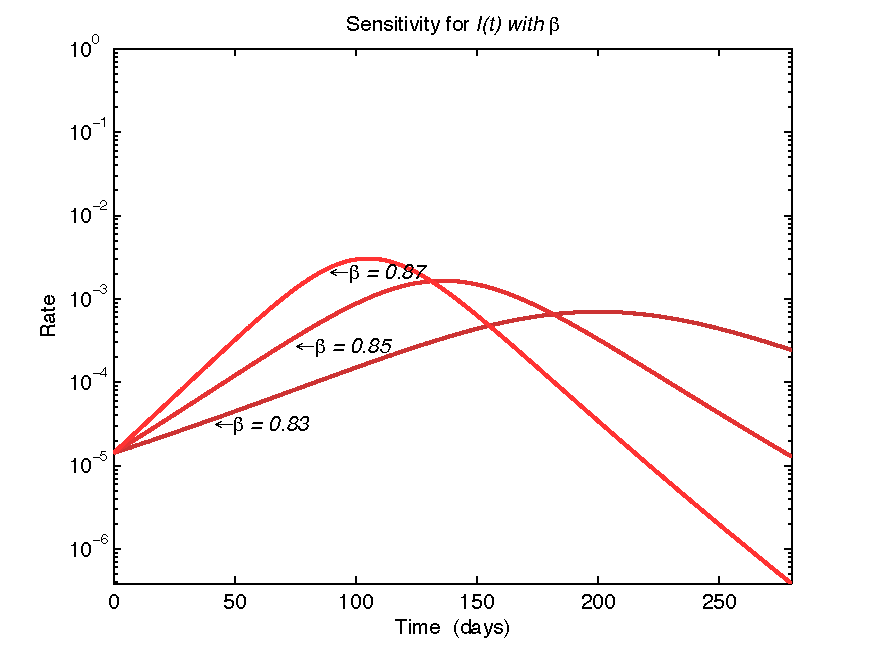
\includegraphics[width=8cm]{figure11.pdf}}
%      \ffigbox{\caption{Sensitivity for $S(t)$ with $\beta$}\label{fig:figure122}}{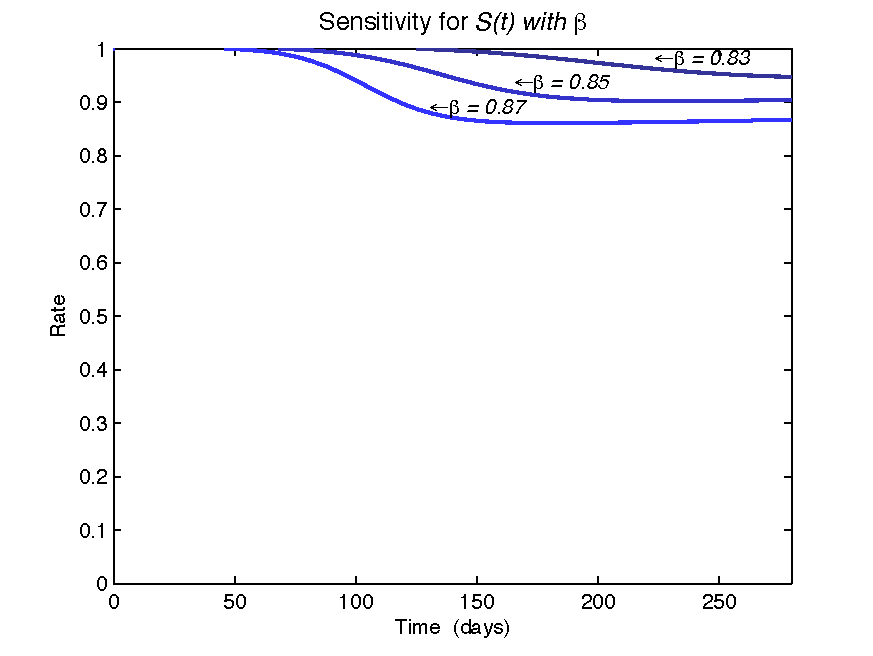
\includegraphics[width=8cm]{figure122.pdf}}
%      \end{floatrow}
%    \end{figure}


\subsection{Strength and weaknesses}

\paragraph{Strength}

Through the theory of AHP, it's not hard to say that our model has the following strength:
\begin{enumerate}
\item Structed. Our model regard the problem as a system, which could be divided and solved by comparison.
\item Practicable. The AHP model combine the methods of quantitative and qualitative. Thus it can deal with realistic problem which may not be solved by traditional theory.
\item Concise. Even people with medium degree of education could understand how this model works and get used of its steps, and the calculation won't be complex.

\end{enumerate}

\paragraph{Weaknesses}


However, there are still some weaknesses. Firstly , deriving fuzzy weights from fuzzy pairwise comparison matrices may be too sophisticated and rare to be applied, while deriving crisp weights from fuzzy pairwise comparison matrices proves to be either invalid or subject to significant drawbacks such as producing multiple even conflict priority vectors for a fuzzy pairwise comparison matrix, leading to distinct conclusions\cite{url11}.

Besides the methods of eigenvector method or LLSM are both computationally simple but they does not reach acceptable values of the optimization criteria as maximum deviation, sum of deviations, etc\cite{url12}.


%\subsection{Other Assumptions}
%\renewcommand{\labelitemi}{\ding{43}}

\section{Conclusion}

The model is based on the real condition and the data given, and we combined them to determine the optimized investment strategy.
\begin{itemize}
\item We formulate a Single imputation with linear regression model to processing the missing data. This step could make sure that our results come from credible data.
\item The ROI for charitable organizations is redefined by elements given in data sets. Through AHP model, the ROI score of each school is figured out. Then we get the schools ranked by ROI score.
\item Combining the ranking result with reality, we determine the concrete investment strategy including the investment list, the amount of each donation and the time duration.
\item The stability of this model is analyzed to see how does this model respond to small changes.

\end{itemize}


%==================Reference===========
\addcontentsline{toc}{section}{Reference}%在目录中添加“	Reference”的标记
\small
\bibliographystyle{plain}
\bibliography{mcmpaper}


%\begin{thebibliography}{99}
%\addcontentsline{toc}{section}{References}
%\bibitem{1} D. E. KNUTH   The \TeX{}book  the American
%Mathematical Society and Addison-Wesley
%Publishing Company , 1984-1986.
%\bibitem{2}Lamport, Leslie,  \LaTeX{}: `` A Document %Preparation System '',
%Addison-Wesley Publishing Company, 1986.
%\bibitem{3}http://www.latexstudio.net/
%\bibitem{4}http://www.chinatex.org/
%\end{thebibliography}

%====================附录导入程序代码==========================================
\newpage
\normalsize
\begin{appendices}
    %\renewcommand{\thesection}{\Alph{chapter}.}

%\section{Letter to the Chief Financial Officer (CFO)}
\section{Letter to the CFO of the Goodgrant Foundation}
%  \begin{center}
%  \textbf{Letter to the Chief Financial Officer (CFO) of the Goodgrant Foundation}
%  \end{center}
  Dear Mr. Alpha Chiang:

Firstly please let us show the greatest respect to all the charitable organizations just like you that working hard for people's happiness and dreams. Education can not only improve students appearance but also change their whole life sometimes. And we both have the same aim now-make sure every dollar invested counts.

In order to achieve this goal, we analyzed the data of thousands of schools in America, including the fundamental information of schools themselves, the performance of under-graduates and the economic situation of graduates. The ROI, is redefined by these three aspects including 12 elements in the data set. And with the ROI defined, we could judge which school have potential to make good use of the investment.

Besides, in order to avoid duplicating the investments and focus of other large grant organizations, we built our own model rather than using the model that has been used by other organizations. May this model provide feasible suggestions for your investment.
As it comes to choose schools from candidates, we finally choose to simulate the AHP model, which can transform the complex problem-distributing weight among elements into comparing every two elements. And we set high ROI to be the aim point, then get the weight allocation among the 12 elements. Then schools are ranked by ROI scores.

Here comes the top 10 schools in the table.
\begin{table}[htbp]
  \centering
  \caption{Top 10 Schools}
    \begin{tabular}{cllr}
    \toprule
    \textbf{UNITID} & \multicolumn{1}{c}{\textbf{INSTNM}} & \multicolumn{1}{c}{\textbf{Score}} & \multicolumn{1}{c}{\textbf{Money}} \\
    \midrule
    232557 & Liberty University & 4.055349646 & 5120877.083 \\
    150987 & Ivy Tech Community College & 3.819812778 & 4823453.813 \\
    132903 & University of Central Florida & 3.735811479 & 4717381.498 \\
    214777 & Pennsylvania State University-Main Campus & 3.700081951 & 4672264.175 \\
    164872 & Boston Architectural College & 3.636278663 & 4591696.819 \\
    109651 & Art Center College of Design & 3.605513625 & 4552848.387 \\
    193900 & New York University & 3.603229283 & 4549963.843 \\
    133979 & Florida Memorial University & 3.596437466 & 4541387.502 \\
    133951 & Florida International University & 3.579236866 & 4519667.511 \\
    123952 & Southern California Institute of Architecture & 3.5691246 & 4506898.286 \\
    \bottomrule
    \end{tabular}%
  \label{tab:top10}%
\end{table}%

As investment is limited to 100 million, we want more schools get benefitted while it's also necessary to make sure every school get enough support. Finally top 22 schools in the table are picked up to get donation distributed in accordance with ROI scores. The investment plan is shown in the table attached.

In conclusion, schools are picked up by ROI potential and the invest amount depends on the scores also. All these are to make sure the investment get more effect on the improvement of students' performance.
  \begin{flushright}
  Sincerely

  MCM team
  \end{flushright}

%    some more text \textcolor[rgb]{0.98,0.00,0.00}{\textbf{Input C++ source:}}
%\lstinputlisting[language=C++]{./code/sudoku.cpp}
\newpage
\section{Source Code}


Algorithm source code and simulation programm used in our model as follow.\\


\textbf{\textcolor[rgb]{0.98,0.00,0.00}{Input matlab source:}}
\lstset{breaklines}%这条命令可以让LaTeX自动将长的代码行换行排版

\lstset{extendedchars=false}%这一条命令可以解决代码跨页时,章节标题,页眉等汉字不显示的问题
\lstinputlisting[language=Matlab]{./code/2016/AHP.m}
%\lstinputlisting[language=Matlab]{./code/2016/costFunctionReg.m}
%\lstinputlisting[language=Matlab]{./code/2016/featureNormalize.m}
\lstinputlisting[language=Matlab]{./code/2016/learningCurve.m}
\lstinputlisting[language=Matlab]{./code/2016/MCM2016.m}
\lstinputlisting[language=Matlab]{./code/2016/MCM2016_AHP.m}
\lstinputlisting[language=Matlab]{./code/2016/validationCurve.m}
%\lstinputlisting[language=Matlab]{./code/calculateDis.m}



\end{appendices}
